\documentclass[a4paper]{article}

\usepackage{amsmath,amssymb,amsfonts}
\usepackage{amssymb, amsmath}
\usepackage{ascmac}
\usepackage{algorithmic}

\DeclareMathOperator{\Bern}{\rm Bern}
\DeclareMathOperator{\Bin}{\rm Bin}
\DeclareMathOperator{\Po}{\rm Po}
\DeclareMathOperator{\Cat}{\rm Cat}
\DeclareMathOperator{\Mult}{\rm Mult}
\DeclareMathOperator{\Beta}{\rm Beta}
\DeclareMathOperator{\Dir}{\rm Dir}
\DeclareMathOperator{\N}{\mathcal{N}}
\DeclareMathOperator{\InvW}{\mathcal{IW}}
\DeclareMathOperator{\NIW}{\mathcal{NIW}}

\newcommand{\proptoas}[1]{\overset{#1}{\propto}}
\DeclareMathOperator{\defeq}{\ensuremath{\stackrel{\mathrm{def}}{=}}}

\usepackage{braket}
\usepackage{url}

\usepackage[dvipdfmx]{graphicx}

\title{Sample of HMM parameters estimation using Gibbs sampling method}
\author{
	Ryo Ozaki\\
	Ritsumeikan University\\
	Graduate School of Information Science and Engineering\\
	Emergent Systems Laboratory\\
	ryo.ozaki@em.ci.ritsumei.ac.jp
}

\begin{document}
\maketitle
\section{Graphical model}
This section shows the graphical model of hidden Markov model (HMM) which were used this paper.
\begin{figure}[ht]
	\begin{center}
		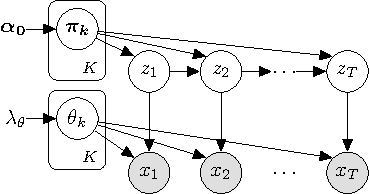
\includegraphics[width=7cm]{fig/HMM_graphical_model.pdf}
		\caption{Graphical model of HMM.}
	\end{center}
\end{figure}

The probabilistic generative process of HMM is shown below.
\begin{eqnarray}
	\boldsymbol{\pi_0} &\sim& \Dir(\boldsymbol{\pi} | \boldsymbol{\alpha_0}) \\
	\boldsymbol{\pi_{k}} &\sim& \Dir(\boldsymbol{\pi} | \boldsymbol{\alpha_0}) \\
	\theta_k &\sim& p(\theta | \lambda_\theta) \\
	z_1 &\sim& \Cat(z | \boldsymbol{\pi_0})\\
	z_t &\sim& \Cat(z | \boldsymbol{\pi_{z_{t-1}}})\\
	x_t &\sim& p(x | \theta_{z_t})\\
	\nonumber \\
	k &=& 1, 2, \ldots, K \\
	t &=& 1, \ldots, T
\end{eqnarray}
Here, $\Dir$ represents the Dirichlet distribution, $\Cat$ represents the categorical distribution.
And, you can use the any emission distribution $p(x | \theta_{t})$ and prior distribution $p(\theta | \lambda_\theta)$.
For example, set $p(x | \theta_{t})$ to multivariate normal distribution and set $p(\theta | \lambda_\theta)$ to normal-inverse-Wishart distribution.

\section{Posterior distribution}
This section shows the posterior distributions.

\subsection{Posterior distribution of $z_t$}
When sample the latent variables sequence, basically we use the blocked Gibbs sampling.
In this section, we shows the sampling algorithm using blocked Gibbs sampling.
\par
In the blocked Gibbs sampling of HMM, the latent variable sequence $z_{1:T}$ are sampled by the conditional posterior distribution $p(z_{1:T} | x_{1:T}, \boldsymbol{\pi_{0:K}}, \theta_{1:K})$.
The distribution is little bit redundancy, so, we don't write the $\boldsymbol{\pi_{0:K}}$ and $\theta_{1:K}$ often in condition part.
Here, $p(z_{1:T} | x_{1:T})$ can be described as follows.
\begin{eqnarray}
	p(z_{1:T} | x_{1:T}) &=& p(z_1 | x_{1:T}) p(z_{2:T} | z_1, x_{1:T}) \\
	&=&
	p(z_1 | x_{1:T}) p(z_2 | z_1, x_{1:T}) p(z_{3:T} | z_1, z_2, x_{1:T}) \\
	&&
	\vdots \\
	&=&
	\prod_{t=1}^{T}{p(z_{t} | z_{1:t-1}, x_{1:T})}
\end{eqnarray}
And then, the term $p(z_{t} = i | z_{1:t-1}, x_{1:T})$ will be calculate as follows.
\begin{eqnarray}
	p(z_{t} = i | z_{1:t-1}, x_{1:T})
	&\proptoas{z_t}&
	p(x_{1:T} | z_{1:t-1}, z_t = i) p(z_t = i | z_{1:t-1})\\
	&=&
	p(x_{1:t-1} | z_{1:t-1}) p(x_{t:T} | z_t = i) p(z_t = i | z_{t-1}) \\
	&\proptoas{z_t}&
	p(x_{t:T} | z_t = i) p(z_t = i | z_{t-1}) \\
	&=&
	p(x_t | z_t = i) p(x_{t+1:T} | z_t = i) p(z_t = i | z_{t-1}) \\
	&=&
	p(x_t | z_t = i) p(z_t = i | z_{t-1}) \beta_t(i)
\end{eqnarray}
Here, $p(x_{t+1:T} | z_t = i)$ is called ``backward message,'' and it defined as $\beta_t(i)$.
And here, latent variables $z_{1:t-1}$ have already been sampled when sampling $z_t$.
Therefore, we can think that latent variables $z_{1:t-1}$ are constant irrespective of $z_t$.
However, you should be care full that the latent variables $z_{t+1:T}$ are still probabilistic variables when sampling $z_t$.
\begin{eqnarray}
	\beta_t(i)
	&\defeq&
	p(x_{t+1:T} | z_t = i)
\end{eqnarray}
And moreover, $\beta_t(i)$ can be calculated recursively.
\begin{eqnarray}
	\beta_t(i)
	&=&
	\sum_{j}{p(x_{t+1:T}, z_{t+1} = j | z_t = i)} \\
	&=&
	\sum_{j}{p(x_{t+1:T} | z_{t+1} = j, z_t = i) p(z_{t+1} = j | z_t = i)} \\
	&=&
	\sum_{j}{p(x_{t+1:T} | z_{t+1} = j) p(z_{t+1} = j | z_t = i)} \\
	&=&
	\sum_{j}{p(x_{t+1} | z_{t+1} = j) p(x_{t+2:T} | z_{t+1} = j) p(z_{t+1} = j | z_t = i)} \\
	&=&
	\sum_{j}{p(x_{t+1} | z_{t+1} = j) p(z_{t+1} = j | z_t = i) \beta_{t+1}(j)}
\end{eqnarray}
In addition, the $\beta_{T-1}(i)$ is equals to as follows, and the initial value $\beta_T(j)$ is as follows.
\begin{eqnarray}
	\beta_{T-1}(i)
	&=&
	\sum_{j}{p(x_{T} | z_{T} = j) p(z_{T} = j | z_{T-1} = i)}\\
	&=&
	\sum_{j}{p(x_{T} | z_{T} = j) p(z_{T} = j | z_{T-1} = i) \beta_T(j)} \\
	\beta_T(j) &=& 1
\end{eqnarray}
Summarize, the posterior distribution of latent variable sequence is as follows.
\begin{eqnarray}
	p(z_{1:T} | x_{1:T})
	&=&
	\prod_{t=1}^{T}{p(z_{t} | z_{1:t-1}, x_{1:T})} \\
	p(z_{t} = i | z_{1:t-1}, x_{1:T})
	&\proptoas{z_t}&
	p(x_t | z_t = i) p(z_t = i | z_{t-1}) \beta_t(i) \\
	\beta_t(i)
	&=&
	\sum_{j}{p(x_{t+1} | z_{t+1} = j) p(z_{t+1} = j | z_t = i) \beta_{t+1}(j)} \nonumber \\
	\\
	\beta_T(i) &=& 1
\end{eqnarray}
Therefore, the posterior distribution of $z_t$ is as follows.
\begin{eqnarray}
	p(z_t = i | x_{1:T}, z_{1:t-1}, \boldsymbol{\pi_{0:K}}, \theta_{1:K})
	\proptoas{z_t} ~~~~~~~~~~~~~~~~~~~~~~~~~~~~~~~~~~~~~~~~~~ \nonumber \\
	p(x_t | z_t = i, \theta_{1:K}) p(z_t = i | z_{t-1}, \boldsymbol{\pi_{0:K}}) \beta_t(i)
\end{eqnarray}
In addition, the array which the value of posterior distribution arranged from $k=1$ to $k=K$ is as follows.
\begin{eqnarray}
	\left[
		\begin{array}{c}
			p(z_t = 1 | x_{1:T}, z_{1:t-1}) \\
			p(z_t = 2 | x_{1:T}, z_{1:t-1}) \\
			\vdots \\
			p(z_t = i | x_{1:T}, z_{1:t-1})
		\end{array}
	\right]
	&=&
	\eta \cdot
	\left[
		\begin{array}{c}
			p(x_t | z_t = 1) p(z_t = 1 | z_{t-1}) \beta_t(1) \\
			\vdots \\
			p(x_t | z_t = i) p(z_t = i | z_{t-1}) \beta_t(i) \\
			\vdots \\
			p(x_t | z_t = K) p(z_t = i | z_{t-1}) \beta_t(K)
		\end{array}
	\right] \nonumber \\
	\nonumber \\
	&\proptoas{z_t}&
	\left[
		\begin{array}{c}
			p(x_t | z_t = 1) p(z_t = 1 | z_{t-1}) \beta_t(1) \\
			\vdots \\
			p(x_t | z_t = i) p(z_t = i | z_{t-1}) \beta_t(i) \\
			\vdots \\
			p(x_t | z_t = K) p(z_t = i | z_{t-1}) \beta_t(K)
		\end{array}
	\right] \nonumber \\
\end{eqnarray}
Here, $\eta$ is defined as the constant term, and it will be able to calculate the value using the restoration.
\begin{eqnarray}
	\eta \cdot \sum_{k=1}^{K}{\left\{p(x_t | z_t = i) p(z_t = i | z_{t-1}) \beta_t(i)\right\}} &=& 1
\end{eqnarray}
\begin{eqnarray}
\eta &=& \frac{1}{\sum_{k=1}^{K}{\left\{p(x_t | z_t = i) p(z_t = i | z_{t-1}) \beta_t(i)\right\}}}
\end{eqnarray}

\subsection{Posterior distribution of $\boldsymbol{\pi_0}$}
The posterior distribution of $\boldsymbol{\pi_0}$ is represented as follows.
\begin{eqnarray}
	p(\boldsymbol{\pi_0} | \boldsymbol{\alpha_0}, \{z_{1:T_s}^{s}\}_{s=1,\ldots,S})
	&=&
	p(\boldsymbol{\pi_0} | \boldsymbol{\alpha_0}, \{z_{1}^{s}\}_{s=1,\ldots,S}) \\
	&\proptoas{\boldsymbol{\pi_0}}&
	p(\{z_{1}^{s}\}_{s=1,\ldots,S} | \boldsymbol{\pi_0}) p(\boldsymbol{\pi_0} | \boldsymbol{\alpha_0})\\
	&=&
	\prod_{s=1}^{S}{\left\{ p(z^{s}_{1} | \boldsymbol{\pi_0}) \right\} } p(\boldsymbol{\pi_0} | \boldsymbol{\alpha_0})\\
	&=&
	\prod_{s=1}^{S}{\left\{ \Cat(z^{s}_{1} | \boldsymbol{\pi_0}) \right\} } \Dir(\boldsymbol{\pi_0} | \boldsymbol{\alpha_0})\\
	&=&
	\Mult(\boldsymbol{m} | \boldsymbol{\pi_0}) \Dir(\boldsymbol{\pi_0} | \boldsymbol{\alpha_0})\\
	&=&
	\Dir(\boldsymbol{\pi} | \boldsymbol{\alpha^*_0})\\
	\nonumber \\
	m_k &=& \sum_{s=1}^{S}{\delta(z^s_1 = i)}\\
	\delta(\text{CONDITION})
	&=&
	\left\{
	\begin{array}{ll}
		0 & (\text{CONDITION is false})\\
		1 & (\text{CONDITION is true})
	\end{array}
	\right.\\
	\nonumber\\
	\boldsymbol{\alpha^*_0} &=& \boldsymbol{m} + \boldsymbol{\alpha_0}
\end{eqnarray}
Here, $S$ represents the number of sequence of $z$, and $z_{1:T_s}^{s}$ represents the $s$-th sequence.
$\Mult$ represents multinomial distribution.

\subsection{Posterior distribution of $\boldsymbol{\pi_k}$}
The posterior distribution of $\boldsymbol{\pi_k}$ is represented as follows.
\begin{eqnarray}
	Z_{k} &=& \Set{z^{s}_{t} | z^{s}_{t-1} = k, s=1,\ldots,S, t=2,\ldots,T_s} \nonumber \\
	\\
	p(\boldsymbol{\pi_k} | \boldsymbol{\alpha_0}, \{z_{1:T_s}^{s}\}_{s=1,\ldots,S})
	&=&
	p(\boldsymbol{\pi_k} | \boldsymbol{\alpha_0}, Z_{k}) \\
	&\proptoas{\boldsymbol{\pi_k}}&
	p(Z_{k} | \boldsymbol{\pi_k}) p(\boldsymbol{\pi_k} | \boldsymbol{\alpha_0})\\
	&=&
	\prod_{z_i \in Z_k}{\left\{ p(z_i | \boldsymbol{\pi_k}) \right\} } p(\boldsymbol{\pi_k} | \boldsymbol{\alpha_0})\\
	&=&
	\prod_{z_i \in Z_k}{\left\{ \Cat(z_i | \boldsymbol{\pi_k}) \right\} } \Dir(\boldsymbol{\pi_k} | \boldsymbol{\alpha_0})\\
	&=&
	\Mult(\boldsymbol{m} | \boldsymbol{\pi_k}) \Dir(\boldsymbol{\pi_k} | \boldsymbol{\alpha_0})\\
	&=&
	\Dir(\boldsymbol{\pi} | \boldsymbol{\alpha^*_k})\\
	\nonumber \\
	m_j &=& \sum_{z_i \in Z_k}{\delta(z_i = j)}\\
	\delta(\text{CONDITION})
	&=&
	\left\{
	\begin{array}{ll}
		0 & (\text{CONDITION is false})\\
		1 & (\text{CONDITION is true})
	\end{array}
	\right.\\
	\nonumber\\
	\boldsymbol{\alpha^*_k} &=& \boldsymbol{m} + \boldsymbol{\alpha_0}
\end{eqnarray}
Here, $\Mult$ represents multinomial distribution.

\subsection{Posterior distribution of $\theta_k$}
The posterior distribution of $\theta_k$ is represented as same as GMM.
So, I do not introduce in here.
Please see GMM.

\newpage
\appendix
\section*{Appendix}
\section{Blocked Gibbs sampling}
In Gibbs sampling, all parameters are sampled by the conditional distribution each other.
For example, the parameters are $\Set{\theta_1, \theta_2, \theta_3}$, we can get the values which sampled by joint distribution $p(\theta_1, \theta_2, \theta_3)$ using each conditional distribution $p(\theta_1 | \theta_2, \theta_3)$, $p(\theta_2 | \theta_1, \theta_3)$, and $p(\theta_3 | \theta_1, \theta_2)$.
\begin{algorithmic}[1]
	\STATE initialize the parameters $\theta_1$, $\theta_2$, and $\theta_3$.
	\WHILE{burn-in loops}
		\STATE $\theta_1 \sim p(\theta_1 | \theta_2, \theta_3)$
		\STATE $\theta_2 \sim p(\theta_2 | \theta_1, \theta_3)$
		\STATE $\theta_ 3\sim p(\theta_3 | \theta_1, \theta_2)$
	\ENDWHILE
	\STATE $(\theta_1, \theta_2, \theta_3)$ are become to values which sampled by $p(\theta_1, \theta_2, \theta_3)$.
\end{algorithmic}
Then, in the blocked Gibbs sampling, some grouped parameters are sampled by conditional joint distribution.
For example, the $\theta_1$ and $\theta_2$ are grouped, the procedure of Gibbs sampling are as follows.
\begin{algorithmic}[1]
	\STATE initialize the parameters $\theta_1$, $\theta_2$, and $\theta_3$.
	\WHILE{burn-in loops}
		\STATE $(\theta_1, \theta_2) \sim p(\theta_1, \theta_2 | \theta_3)$
		\STATE $\theta_ 3\sim p(\theta_3 | \theta_1, \theta_2)$
	\ENDWHILE
	\STATE $(\theta_1, \theta_2, \theta_3)$ are become to values which sampled by $p(\theta_1, \theta_2, \theta_3)$.
\end{algorithmic}
In addition, the conditional joint distribution $p(\theta_1, \theta_2 | \theta_3)$ are divided to as follows:
\begin{eqnarray}
p(\theta_1, \theta_2 | \theta_3) &=& p(\theta_1 | \theta_3) p(\theta_2 | \theta_1, \theta_3).
\end{eqnarray}
And, the marginal distribution $p(\theta_1 | \theta_3)$ are calculated by
\begin{eqnarray}
p(\theta_1 | \theta_3) &=& \int{p(\theta_1 , \theta_2 | \theta_3) d\theta_2}
\end{eqnarray}

\section{Scaling the backward message}
In the Gibbs sampling of HMM, we calculated the backward message as follows.
\begin{eqnarray}
	\beta_t(i) &=& \sum_{j}{p(x_{t+1} | z_{t+1} = j) p(z_{t+1} = j | z_{t} = i) \beta_{t+1}(j)} \\
	\beta_T(i) &=& 1
\end{eqnarray}
And the backward message was used to sampling the hidden state sequence as follows.
\begin{eqnarray}
	p(z_{t} = i | z_{1:t-1}, x_{1:T})
	&\proptoas{z_t}&
	p(x_t | z_t = i) p(z_t = i | z_{t-1}) \beta_t(i)
\end{eqnarray}
Here, the backward message will be becoming to very small values, because, the backward message was calculated by many products of probability which value is less than 1.
The case of the sequence length is very long, the value of the backward message might not be able to calculate because of underflow.
So, we need to scaling the backward message.
In this section, I will be introducing the 2 way to scaling backward message.

\subsection{Log scaling}
Using log scale is the very popular way to keep the small value without underflow as the classical method.
After taking the log scale of backward message is as follows.
\begin{eqnarray}
	E_{t}(j) &=& \log{p(x_{t} | z_{t} = j)}\\
	A_{t}(i, j) &=& \log{p(z_t = j | z_{t-1} = i)}\\
	B_t(i) &=& \log{\beta_t(i)}\\
	\nonumber \\
	B_t(i) &=& \log{\left[\sum_{j}{\exp{ \left\{ E_{t+1}(j) + A_{t+1}(i, j) + B_{t+1}(i) \right\}}}\right]} \\
	B_T(i) &=& 0
\end{eqnarray}
In addition, the format of calculating formula $B(z_t)$ is called ``LogSumExp.''
The LogSumExp is calculated by as follows.
\begin{eqnarray}
	y &=& \log{\left\{ \exp{(x_1)} + \ldots + \exp{(x_n)} \right\}} \\
	&=& \log{\left\{ \exp{(x^*)} \left( \exp{(x_1 - x^*)} + \ldots + \exp{(x_n - x^*)} \right)\right\}} \\
	&=& x^* + \log{\left\{ \exp{(x_1 - x^*)} + \ldots + \exp{(x_n - x^*)} \right\}} \\
	x^* &=& \max{\{ x_1, \ldots, x_n \}}
\end{eqnarray}
By this calculating, the risk of underflow is low, because, the $|x_i - x^*|$ is small than $|x_i|$.
In addition, it needs to take exp when sampling the hidden state $z_t$, but, it needs only the information about proportional.
Therefore, the posterior distribution of the hidden state $z_t$ is represented as follows.
\begin{eqnarray}
	p(z_{t} = i | z_{1:t-1}, x_{1:T})
	&\proptoas{z_t}&
	p(x_t | z_t = i) p(z_t = i | z_{t-1}) \exp{\left(B_t(i)\right)} \\
	&\proptoas{z_t}&
	p(x_t | z_t = i) p(z_t = i | z_{t-1}) \exp{\left(B_t(i) - B_{MAX}\right)} \\
	\nonumber \\
	B_{MAX} &=& \max{\left\{ B_t(1), B_t(2), \ldots, B_t(K)\right\}}
\end{eqnarray}

\subsection{Normalizing}
In normalizing, calculating the proportional value of a backward message as follows.
\begin{eqnarray}
	\hat{\beta}_t(i) &=& \frac{1}{c_t} \beta_t(i) \\
	&\proptoas{z_t}& \beta_t(i)
\end{eqnarray}
Here, $c_t$ is a normalizing constant.
The $c_t$ is calculated by some restriction.
In this section, we set the restriction to the max value of the $\hat{\beta}_t(i)$ is 1.
\begin{eqnarray}
	c_t &=& \max{\left\{ \beta_t(1), \beta_t(2), \ldots, \beta_t(K)\right\}}
\end{eqnarray}
After this representation, the backward message is as follows.
\begin{eqnarray}
	\hat{\beta}_t(i) &=& \frac{c_{t+1}}{c_t} \sum_{j}{p(x_{t+1} | z_{t+1} = j) p(z_{t+1} = j | z_{t} = i) \hat{\beta}_{t+1}(j)} \\
	\hat{\beta}_T(i) &=& 1
\end{eqnarray}
Here, we need to calculate the normalization term $\frac{c_{t+1}}{c_t}$.
And the normalization term is normalizing the max value to 1.
Therefore, the value of $\frac{c_{t+1}}{c_t}$ is as follows.
\begin{eqnarray}
	\hat{\beta}_{t}^{-}(i)
	&=&
	\sum_{j}{p(x_{t+1} | z_{t+1} = j) p(z_{t+1} = j | z_{t} = i) \hat{\beta}_{t+1}(j)} \\
	\left(\frac{c_{t+1}}{c_t}\right)^{-1}
	&=&
	\max{\left\{ \hat{\beta}_{t}^{-}(1), \hat{\beta}_{t}^{-}(2), \ldots, \hat{\beta}_{t}^{-}(K)\right\}}
\end{eqnarray}
Finally, the posterior distribution of $z_t$ is as follows.
\begin{eqnarray}
	p(z_{t} = i | z_{1:t-1}, x_{1:T})
	&\proptoas{z_t}&
	p(x_t | z_t = i) p(z_t = i | z_{t-1}) \beta_t(i) \\
	&\proptoas{z_t}&
	p(x_t | z_t) p(z_t | z_{t-1}) \hat{\beta}_t(i)
\end{eqnarray}
If you want to use another restriction, you have to care the initial value of backward message.
E.g.,
\begin{eqnarray}
	c_t &=& \sum_{k=1}^{K}{\beta_t(k)} \\
	\hat{\beta}_T(i) &=& \frac{1}{K}\\
	\left(\frac{c_{t+1}}{c_t}\right)^{-1} &=& \sum_{k=1}^{K}{\hat{\beta}_{t}^{-}(k)}
\end{eqnarray}
\end{document}
